\section{Politiche di sicurezza}
Gli e-commerce, più di molti altri siti web, devono garantire un livello di sicurezza più che eccellente in quanto le conseguenze causate da eventuali bug o vulnerabilità sono potenzialmente catastrofiche per gli utenti che usufruiscono della piattaforma. All'interno del ciclo di vita del software l'azienda deve definire delle rigide politiche di sicurezza volte a garantire la continuità operativa e la riservatezza delle informazioni associate agli utenti. Ho quindi definito ed adottato le seguenti politiche di sicurezza: 
\begin{itemize}
    \item \textbf{Rinominare con nomi casuali i file caricati dagli utenti}, degli eventuali attaccanti possono caricare file con nomi particolari volti ad accedere a cartelle contenenti file sensibili che quindi risulterebbero compromessi; 
    \item \textbf{Controllare il contenuto dei file caricati dagli utenti}, gli unici file che gli utenti possono caricare sono le immagini, viene quindi fatto un doppio controllo (lato client e lato server) per assicurarsi che i file caricati rispettino il corretto formato; 
    \item \textbf{Uso del pattern Post/Redirect/Get}, questo pattern particolare adottato in maniera estensiva nel web permette di ovviare al problema della ricarica o navigazione temporale delle pagine e richieste già inviate al server \cite{PRG}. Seguendo questo pattern tutte le richieste POST verranno prima elaborate e poi reindirizzate su la stessa o un'altra pagina che verrà ottenuta tramite richiesta GET, in questo modo l'utente nella sua navigazione non incontrerà mai messaggi relativi alla celebre "Conferma reinvio modulo"; 
    \item \textbf{HTTPS} \cite{HTTPS}, il sito usa il protocollo TLS/SSL insieme al protocollo HTTP per la navigazione sicura all'interno del sito, i dati trasmessi da e verso il sito attraversano un tunnel end-to-end dentro il quale sono crittografati e non leggibili da possibili attaccanti; 
    \item \textbf{Autenticazione degli utenti}, gli utenti si devono autenticare per poter compiere azioni sul sito come inserire un prodotto; 
    \item \textbf{Password hashing}, le password usate dagli utenti non vengono salvate in chiaro dal database che invece le memorizza già crittografate;
    \item \textbf{Uso di un Firewall}, i dispositivi essendo connessi in rete possono anche essere soggetti di attacchi informatici basati sull'invio di pacchetti maliziosi, l'uso di un Firewall permette di bloccare questi pacchetti e garantire una connessione sicura.  
\end{itemize} 
\subsection{Autenticazione}
La piattaforma ha due modalità di accesso: il sito web e l'API. Entrambe le modalità devono effettuare l'autenticazione dell'utente che s'interfaccia con la piattaforma Rius.Co. verificandone l'identità. 
\medskip

Il sito web si occupa dell'autenticazione richiedendo agli utenti di impostare una password di lunghezza variabile tra gli 8 e i 24 caratteri. I clienti possono anche richiedere la modifica della password che è comunque una pratica da fare periodicamente per evitare problemi relativi alla sicurezza del profilo. 
\medskip

L'API invece esegue l'autenticazione dell'utente in tutt'altro modo, gli utenti alla registrazione ricevono una chiave univoca privata non modificabile (API key) di 32 byte che viene generata in modo casuale \cite{APIKEY}. Questa chiave dovrà quindi essere inserita nel form di tutte le richieste fatte all'API per permettere l'identificazione dell'utente associato alla richiesta. Alcune richieste come ottenere un file in formato JSON contenente tutti i prodotti presenti sul Marketplace non necessitano dell'autenticazione e vengono eseguite anche senza l'API key in quanto sono informazioni pubbliche visualizzabili da chiunque. 
\bigskip

\textbf{Esempio di richiesta con autenticazione all'API tramite curl}
\begin{lstlisting}[style=dos]
$ curl -X GET --insecure "https://0.0.0.0:6066/Transactions/GetTransactionsByUserID/9" -F  "apiKey=aBQKfxy175kL1v5EdOwCkHWtgwAj9Kbzu339OkDIgxA="
\end{lstlisting}
\bigskip

\textbf{Risposta del server in formato JSON contenente tutte le transazioni in cui ha partecipato l'utente con l'API key indicata} 
\lstinputlisting[style=json]{content/code/response.json}
\subsection{Password hashing} 
Per garantire la privacy degli utenti ed evitare che i profili vengano violati in caso di data breach o altri tipi di fughe di informazioni è necessario rendere praticamente impossibile ottenere le password impostate dagli utenti. Le password devono quindi essere crittografate con algoritmi che rendano impraticabile la decifrazione anche in caso di attacchi come il brute-force. Per la piattaforma Rius.Co. ho deciso di usare gli standard più recenti e robusti dal punto di vista informatico per eseguire l'hashing di tutte le password. L'hashing consiste nel produrre una stringa o digest correlata ad una serie di dati che sono in questo caso la password, una buona funzione di hashing rende praticamente impossibile risalire alla password partendo dal digest ma restituisce sempre lo stesso digest nel caso venga usata la stessa password \cite{Hashing}. In questo modo nel database è riportata solo l'elaborazione della password dalla quale nessuno può risalire all'originale.
\medskip

Per eseguire l'hashing delle password ho implementato la funzione di derivazione della chiave consigliata sia da Microsoft \cite{HashingASPNET} che dal RFC 8018 \cite{RFC8018}, questa è definita nel RFC 2898 \cite{RFC2898} e prende il nome di PBKDF2 (Password-Based Key Derivation Function 2) \cite{PBKDF2}. Questa funzione è ritenuta la migliore dal punto di vista di semplicità, prestazioni e sicurezza; restituisce una chiave derivata (DK) che equivale all'hash della password ed è rappresentata in questo modo:

\begin{center}
    \begin{lstlisting}
        DK = PBKDF2(PRF, Password, Salt, c, dkLen) 
    \end{lstlisting}
\end{center}
\clearpage

Per ottenere la chiave derivata sono quindi richiesti i seguenti parametri: 
\begin{itemize}
    \item PRF, la funzione pseudocasuale che si occuperà ad ogni iterazione di eseguire l'hashing dei dati con la generazione del Message Authentication Code (HMAC);
    \item Password, la password della quale eseguire l'hashing e ottenerne la chiave derivata;
    \item Salt, una sequenza casuale di byte assegnata automaticamente all'utente e salvata in chiaro nel database. Il salt viene sommato alla password dell'utente prima dell'hashing per far sì che due password uguali di due utenti diversi producano hash altrettanto diversi, rendendo ancora più difficile la decifrazione tramite brute-force \cite{Salt};
    \item c, il numero di iterazioni da svolgere per ottenere la chiave derivata, l'aumentare del numero di iterazioni comporta l'importante aumento sia del livello di sicurezza che del tempo di esecuzione della funzione che perde in velocità;
    \item dkLen, la lunghezza in byte della chiave derivata.
\end{itemize}
\medskip

\begin{figure}[ht]
    \centering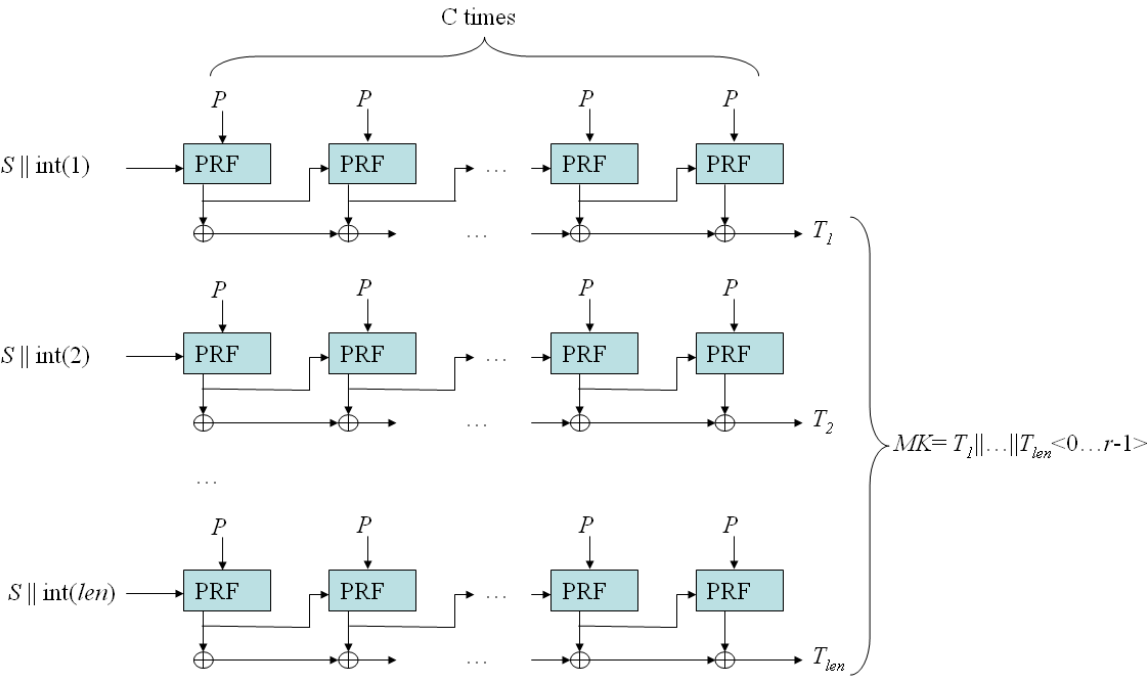
\includegraphics[scale=0.44]{images/Pbkdf2.png}
    \caption{Rappresentazione grafica dell'algoritmo che compone un'iterazione.}
\end{figure}

\medskip
Nella mia funzione GetHash PBKDF2 esegue 10000 iterazioni con l'algoritmo di hashing HMACSHA256, usa un Salt di 128 byte, e produce un'elaborazione della password lunga 32 byte. 
\smallskip

\begin{lstlisting}[style=csharp]
private static string GetHash(string password, string salt)
{
    return Convert.ToBase64String(KeyDerivation.Pbkdf2(
        password: password,
        salt: Encoding.UTF8.GetBytes(salt),
        prf: KeyDerivationPrf.HMACSHA256,
        iterationCount: 10000,
        numBytesRequested: 32));
}
\end{lstlisting}
\subsection{Firewall}
Un firewall consiste in un componente hardware o software che si occupa della difesa di una rete, questo analizza i pacchetti in entrata ed uscita e attraverso le regole fornite dall'amministratore di rete decide se permettere o bloccare il passaggio di questi pacchetti \cite{Firewall}. Le regole prendono il nome di access-list e definiscono il traffico che ha il permesso di attraversare la rete. Nel caso dell'infrastruttura sulla quale si appoggia Rius.Co. sono presenti due router che svolgono entrambi anche la funzione di firewall, questi sono collocati al bordo delle due reti, ovvero quella aziendale e quella contenente i server. Nel router di bordo collocato nella rete dei server il traffico nella sua completezza è permesso solo dalla rete aziendale, sono state però impostate due access-list per permettere l'accesso all'API server e al Web server che devono poter essere raggiungibili da chiunque. 
\bigskip

\textbf{Configurazione del firewall collocato sul router di bordo della rete VPC con indirizzo IP pubblico 1.0.0.1}
\begin{lstlisting}[style=dos]
    interface GigabitEthernet0/0
        ip address 1.0.0.1 255.0.0.0
        ip access-group 101 in
        
    access-list 101 permit ip any host 192.168.1.5
    access-list 101 permit ip any host 192.168.1.3
    access-list 101 permit ip 192.168.0.0 0.0.255.255 any
    access-list 101 deny ip any any
\end{lstlisting}
